\begin{figure}[hbtp]
  \centering
  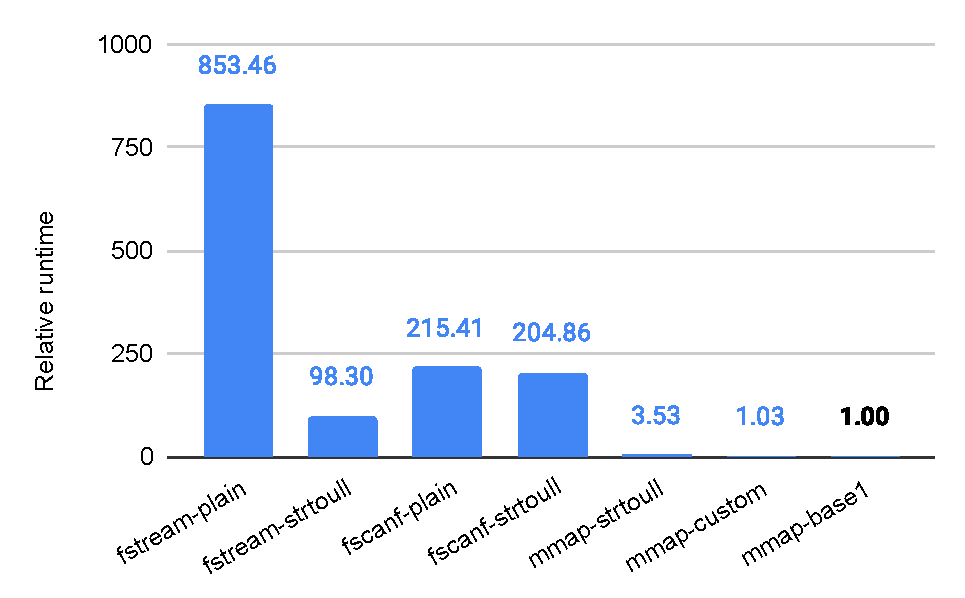
\includegraphics[width=0.99\linewidth]{out/optimize-el.pdf} \\[-2ex]
  \caption{Relative runtime of reading per-thread edge-lists using C++'s input file stream (\textit{fstream-plain}), file stream to read lines and using  \texttt{strtoull} and \texttt{strtod} function for parsing numbers (\textit{fstream-strtoull}), \texttt{fgets} to read lines and \texttt{sscanf} for parsing numbers (\textit{fscanf-plain}), \texttt{fgets} with \texttt{strtoull} and \texttt{strtod} (\textit{fscanf-strtoull}), memory mapped file using \texttt{mmap} with \texttt{strtoull} and \texttt{strtod} (\textit{mmap-strtoull}), \texttt{mmap} with custom integer/float parsing functions (\textit{mmap-custom}), and \texttt{mmap} with custom integer/float parsing functions along with making vertex id 0-based (\textit{mmap-base1}).}
  \label{fig:optimize-el}
\end{figure}
